\documentclass[aps, pra, 10pt, twocolumn, superscriptaddress,floatfix]{revtex4-1}

\usepackage{amsmath,amssymb,amsfonts}
\usepackage{braket}
\usepackage[breaklinks=true,colorlinks,citecolor=blue,linkcolor=blue,urlcolor=blue]{hyperref}
\usepackage{mathtools}
\usepackage{dsfont}

%%
\def \id {\mathds{1}}
\def \abs {\text{Abs}}
\newcommand{\norm}[1]{\lVert#1\rVert}
\DeclareMathOperator{\tr}{Tr}
\newcommand{\round}[1]{\ensuremath{\lfloor#1\rceil}}
\newcommand{\mi}{\mathrm{i}} %% roman "i"
%

\begin{abstract}
	In a previous work we have been using an optical platform to test an offline metrological protocol for the estimation of a rotation angle at the Heisenberg scaling. In this notes we deal with the two problems of estimating a phase on the same setup when the visibilities are unknown and therefore are treated as \textit{nuisance} parameters, and the problem of determining one or more visibilities of the optical components (q-plates) of the setup together with the rotation angle. The figure of merit for the error is designed to be robust to the outliers and the experimental results will be compared to a reference value derived from the Cramér-Rao bound.
	
\end{abstract}

\begin{document}
%
\title{Characterization of a metrological optical setup with nuisance parameters} 
%
\author{Federico Belliardo}
\email{federico.belliardo@sns.it}
\affiliation{NEST, Scuola Normale Superiore, I-56126 Pisa,~Italy}

\maketitle


\section{Introduction}
\label{sec:introduction}
%
In this work we want to study the complete characterization of an optical setup, that might be later used by the experimentalists to carry out quantum protocols. We are going to employ the q-plate setup of~\cite{Cimini2021} with three q-plates. This means the apparatus will be characterized by four visibilities: one for the configuration without active q-plates and three for the three configurations with only one q-plate active each. Therefore the parameters to estimate are a rotation angle $\theta \in [0, \pi)$ and the four visibilities $V_1, V_2, V_3, V_4 \in [0, 1]$. In all the Bayesian experiments performed here the prior distributions on the visibilities will be uniform in $[0, 1]$, like the prior on the phase which is uniform in $[0, \pi)$. The Bayesian procedure will be implemented as presented in~\cite{Granade2012} with a particle filter. This method selects the next measurement to be done (the next q-plate) according to the posterior probability distribution for the unknown phase and visibilities. We will first measure only the phase $\theta$ treating the visibilities as \textit{nuisance} parameters. That means our goal will first be the minimization of the variance on the phase only. Here the estimators for the visibilities should be only precise enough to allow us to find a good strategy for the estimation of the phase. Then we will minimize the error on a couple of parameters, that is the phase and one of the visibilities: $(\theta, V_i)$ with $i=1, 2, 3, 4$, the other three visibilities will be again nuisance parameters. At the end we try to estimate all the five parameters $(\theta, V_1, V_2, V_3, V_4)$ at the same time. 

\section{The Bayesian procedure}
\label{sec:bayesian}
%
In this section we present the Bayesian algorithm proposed in~\cite{Granade2012}, with the application to our q-plates setup in mind. With respect to the original formulation we made a few corrections necessary because of the circular nature of the angular variable that we are going to measure. In every experiment $n_p = 5000$ particles have been used. The parameters to estimate are collected in the vector $\boldsymbol{x} := \left( \theta, V_1, V_2, V_3, V_4 \right)$, that contains the phase in the first entry and the four visibilities in the other ones. Being the Granade's method based on a particle filter, it represents internally the posterior probability distribution with the ensemble $\mathcal{E} := \lbrace \boldsymbol{x}^i, w^i \rbrace$, where $\boldsymbol{x}^i$ is the position of the $i$-th particle and $w^i$ its weight. The $j$-th component of the $i$-th particle of the ensemble will be represented as $x_j^i$, and could correspond to the phase if $j=0$, that is $x^i_0 = \theta^i$ or to one of the visibilities if $j=1, 2, 3, 4$, that is $x^i_j = V^i_j$. The mean of the angular values is computed as
%
\begin{equation}
	\hat{\mu}_0 := \arg \left[ \sum_{i=1}^{n_{p}} w^i \exp \left( \mi \theta^i \right) \right] \; ,
\end{equation}
%
while the mean values of the visibilities are
%
\begin{equation}
	\hat{\mu}_j = \sum_{i=1}^{n_p} w^i V^i_j \; .
\end{equation}
%
Together they form the vectorial mean of the distribution $\boldsymbol{\hat{\mu}} = (\hat{\mu}_0, \hat{\mu}_1, \hat{\mu}_2, \hat{\mu}_3, \hat{\mu}_4)$. The covariance matrix is defined as
%
\begin{equation}
	\text{Cov}_{ij} := \sum_{k=1}^{n_{p}} w^k (x^k_i - \hat{\mu}_i)  (x^k_j - \hat{\mu}_j) \; .
\end{equation}
%
If $i=1$ or $j=1$ then difference in $x^k_i - \hat{\mu}_i$ or $x^k_j - \hat{\mu}_j$ is actually the circular distance
%
\begin{equation}
	d(x^k_i, \hat{\mu}_i) = \pi - | (x^k_i - \hat{\mu}_i) \mod 2 \pi - \pi| \; .
\end{equation}
%
The Bayesian algorithm tries for each new experiment (each new photon sent with a specific q-plate activated) to minimize the scalar variance of the posterior distribution, that is
%
\begin{equation}
	\sigma^2 := \tr \left[ G \cdot \text{Cov} \right] = \sum_{i, j} G_{ij} \text{Cov}_{ij} \; ,
\end{equation}
%
where $G$ is the weight matrix that controls which parameters are to be treated as nuisance parameters. In this way the algorithm attempts to concentrate as much as possible the distribution around its mean in a greedy fashion. The resampling strategy of the Granade procedure has also undergone minor changes to adapt it to the phase estimation problem. The Bayesian data analysis has been performed on the data collected for for $17$ angles chosen uniformly in $[0, \pi)$.
%
\section{Figure of merit for the error}
\label{sec:precision}
%
In this section we will suppose the objective of the estimation are to be the phase $\theta$ and one of the visibilities $V$. The most common figure of merit for the precision of an estimator is the Mean Square Error. Given $\hat{\theta}$ and $\hat{V}$ estimators for $\theta$ and $V$ respectively, their MSE are
%
\begin{eqnarray}
	\Delta^2 \hat{\theta} = \mathbb{E}_{p(\hat{\theta} | \theta)} [|\hat{\theta}-\theta|^2] \; , \\
	\Delta^2 \hat{V} = \mathbb{E}_{p(\hat{V}|\theta)} [|\hat{V}-V|^2] \; ,
\end{eqnarray}
%
where the expectation values are defined as  $\mathbb{E}_{p(\hat{\theta} | \theta)} [...]  := \int d \hat{\theta} ... p(\hat{\theta} | \theta)$ and $\mathbb{E}_{p(\hat{V} | \theta)} [...]  := \int d \hat{V} ... p(\hat{\theta}|\theta)$, being $p(\hat{\theta}|\theta)$ and $p(\hat{V}|\theta)$ the marginals of the joint probability distribution $p(\hat{\theta}, \hat{V}|\theta)$ for $\hat{\theta}$ and $\hat{V}$. The joint error would be $\Delta^2 \hat{\theta} + \Delta^2 \hat{V}$ and could be written as
%
\begin{equation}
	\Delta^2 \hat{\theta} + \Delta^2 \hat{V} = \mathbb{E}_{p(\hat{\theta}, \hat{V}| \theta)} [|\hat{\theta}-\theta|^2 + |\hat{V}-V|^2]
\end{equation}
%
where $\mathbb{E}_{p(\hat{\theta}, \hat{V}| \theta)} [...]  := \int d \hat{\theta} d \hat{V} ... p(\hat{\theta}, \hat{V} | \theta)$. We then consider the expectation value of $	\Delta^2 \hat{\theta} + \Delta^2 \hat{V}$ on the prior probability distribution for $\theta$, that in the following we will assume uniform, i.e.
%
\begin{equation}
	\mathbb{E}_\theta[\Delta^2 \hat{\theta} + \Delta^2 \hat{V}] = \mathbb{E}_\theta \left[ \mathbb{E}_{p(\hat{V}, \hat{\theta}|\theta)} [|\hat{\theta}-\theta|^2 + |\hat{V}-V|^2] \right] \; .
\end{equation}
%
The expectation value on $\theta$ can be approximated the uniform sampling of $J = 17$ angle in $[0, \pi]$, which would give
%
\begin{eqnarray}
	&\frac{1}{J} \sum_{j=1}^J \mathbb{E}_{p(\hat{\theta}, \hat{V} | \theta)} [|\hat{\theta}_j-\theta_j|^2 + |\hat{V}_j-V_j|^2] \\ = 
	&\mathbb{E}_{h} \left[ \frac{1}{J} \sum_{j=1}^J  [|\hat{\theta}_j-\theta_j|^2 + |\hat{V}_j-V_j|^2] \right]  \; .
	\label{eq:hmean}
\end{eqnarray}
%
where 
%
\begin{eqnarray}
	h(\hat{\theta}_1, \dots, \hat{\theta}_J, \hat{V}_1, \dots, \hat{V}_J) = \prod_{j=1}^J p(\hat{\theta}_j, \hat{V}_j | \theta_j) \; .
	\label{eq:hdistr}
\end{eqnarray}
%

However only the marginals $p(\hat{\theta})$ and $p(\hat{V})$ are important in our computation, since we are not considering the correlation between $\hat{\theta}$ and $\hat{V}$. For our purposes we could has well have defined
\begin{eqnarray}
	h(\hat{\theta}_1, \dots, \hat{\theta}_J, \hat{V}_1, \dots, \hat{V}_J) = \prod_{j=1}^J p(\hat{\theta}_j | \theta_j) p(\hat{V}_j | \theta_j) \; .
\end{eqnarray}
%
We need to sample from the distribution $h$, in order to approximate the expectation value in Eq.~\eqref{eq:hmean}. This quantity (which is basically the sample estimator for the Mean Square Error) is however very sensible to outliers, and the Bayesian algorithm produces many of them, since the heavy tails of the estimator $\hat{\theta}$ are not controlled analytically as done in~\cite{Cimini2021}. To circumvent this problem we substitute the expectation value on $h$ with the median, which is much less sensible to outliers. Therefore our figure of merit for the error, which is constructed with the results of the actual experiments and plotted in Sec.~\ref{sec:results}, will be  
%
\begin{equation}
	\text{Median} \left[ \frac{1}{J} \sum_{j=1}^J  [|\hat{\theta}_j-\theta_j|^2 + |\hat{V}_j-V_j|^2] \right] \; .
	\label{eq:medianMerit}
\end{equation}
%
If the only objective of the estimation is the phase $\theta$ then the figure of merit reads
%
\begin{equation}
	\text{Median} \left[ \frac{1}{J} \sum_{j=1}^J  [|\hat{\theta}_j-\theta_j|^2 \right] \; ,
	\label{eq:medianMeritOnlyTheta}
\end{equation}
%
while if all the five parameters $(\theta, V_1, V_2, V_3, V_4)$ are objective of the estimation then we consider
%
\begin{equation}
	\text{Median} \left[ \frac{1}{J} \sum_{j=1}^J \left( [|\hat{\theta}_j-\theta_j|^2 + \sum_{i=1}^4 |\hat{V}_j^i-V^i_j|^2] \right)\right] \; .
	\label{eq:medianMeritAll}
\end{equation}


\section{Details of the algorithm}
%
At difference with the offline algorithm we can't perform the estimation with a fixed number $N$ of total used resources, because the number of photons to use for each q-plate is a stochastic variable, this makes $N$ a stochastic variable too. Only the total number of used photons can be fixed. In order to give a synthetic representation of the performances of the Bayesian method we proceed as following. For each phase, with fixed visibilities, we perform (in parallel) $b$ estimation of the parameters of interest, for example the phase $\theta$ and one of the visibilities $V$, and save for each estimation in the batch at each step the values of the current estimators $\hat{\theta}$, $\hat{V}$, and the number of resources used up to that point, i.e.
%
\begin{equation}
	N := 2 \sum_{i=1}^4 s_i \nu_i \; ,
\end{equation}
%
with $\nu_i$ being the number of photons used for the q-plate with charge $s_i$. An array of length $N_{\max} = 30000$ is loaded with this data. To compute the square deviation we should subtract from this array an array of true values for the phase and the visibilities. The true value of the phase is known with high precision, because it is the rotation angle of the decoding stage, while the visibilities of the q-plates may not be known with comparable precision. For each experiment with a certain $G$ weight matrix as objective and for each phase the true value of the visibility of each q-plate is taken to be the output of the Bayesian algorithm for the maximum number of resources we have considered ($N = 30000$) averaged over the batch of $b$ experiments. According to this the true visibility of a q-plate may be a function of the rotation angle. From $N=100$ to the end of the array the data are clustered, that means we consider all the measurements consuming a number of resources falling in $[N, N+\Delta N]$, with $\Delta N = 50$, as if they were performed with the same resource number and use them to compute the error. The point with $N \le 100$ are not clustered. In principle all the clusters we have build this way could contain a different number of data points. For each cluster (or points with $N \le 100$) we perform a resampling of the estimators, that means we sample $b'$ new points uniformity from the estimators that have fallen in that cluster, so that all the clusters and the points before the cut at $N=100$ have the same number of points $b'$ at the end. We then compute the sum of the square deviations for the parameters of interest $\theta$ and $V$, and build a vector of $b'$ squared deviations $|\hat{\theta} - \theta|^2 + |\hat{V} - V|^2$. This procedure is repeated for each of the $J=17$ phases of the measurement set, that are chosen uniformly in $\left[0, \pi \right)$, and the mean of this values is computed
%
\begin{equation}
	\frac{1}{J} \sum_{j=1}^J |\hat{\theta}_j - \theta_j|^2 + |\hat{V} - V_j|^2 \; .
\end{equation}
%
This procedure has given us $b'$ samples from the distribution in Eq.~\eqref{eq:hdistr} for each cluster of the total resources $N$, and by taking the sample median of them we approximate Eq.~\eqref{eq:medianMerit}. The (asymmetric) confidence interval for the median of each total resources cluster is evaluated with a bootstrap procedure for a $99\%$ confidence level. The point having $N > 100$ should also be given an error bar on the x-axis, of size $\sim \Delta N$, this should be irrelevant for very large $N$, but important for $N \sim \mathcal{O} (100)$, however we have chosen not to plot this error to keep the plots simpler. The number of estimations to be performed in parallel $b$ is to be changed in accordance with the objective of the estimation. The choice of $b$ must guarantee that in every cluster before the resampling there are at least $b' = 200$ points, so that the resampling doesn't artificially reduce the error.

\section{Bayesian Cramér-Rao bound}
%
In this section we formulate a Bayesian Cramér-Rao bound first for the Mean Square Error in Eq.~\eqref{eq:hmean}, and then we modify it to find a reference error for the figure of merit of Eq.~\eqref{eq:medianMerit}, against which the experimental data can be compared. In this section the visibilities $V$ of the q-plates are independent on $\theta$ and are averaged across all the measured phases, this is done to simplify the analytical expressions. The true value of the visibilities are therefore $V_1 = 0.915$, $V_2 = 0.918$, $V_3 = 0.830$, and $V_4 = 0.765$. Consider $\nu$ repetitions of a couple of Type-$0$ and Type-$+$ measurements~\cite{Belliardo2020} performed with a certain q-plate of charge $s$, that produce two results $c_1, c_2 \in \lbrace -1, +1 \rbrace$ each, extracted from the following two probability distribution
%
\begin{equation}
p_1(c_1; \theta, V) = \frac{1 + c_1 \cdot V \cos s \theta}{2} \; ,
\end{equation}
%
and 
%
\begin{equation}
p_2(c_2; \theta, V) = \frac{1 + c_2 \cdot V \sin s \theta}{2} \; .
\end{equation}
%
Our goal is to bound the precision of the joint estimation of $V$ and $\theta$. With this goal we compute the Fisher information matrix for this two measurements respectively, which we call respectively $I_0 (\theta, V)$ and $I_+ (\theta, V)$, and sum them to get $I(\theta, V) := I_0 (\theta, V) + I_+ (\theta, V)$. We obtain the total Fisher information matrix for the angle and the visibilities of all the q-plates by summing the FI matrices corresponding to each quantum resource $s$, for a number $\nu_i$ of couple respectively. It is important that we think $I_i (\theta, V_i)$ as a $5 \times 5$ matrix even if only four entries for each matrix will be non null. In this way we can write the $5 \times 5$ FI matrix for the five parameters $(\theta, V_1, V_2, V_3, V_4)$ as
%
\begin{equation}
I(\theta, V_1, V_2, V_3, V_4) := \sum_{i=1}^4 \nu_i I_i (\theta, V_i) \; .
\end{equation}
%
We report in the following all the non-zero entries of this matrix.
%
\begin{align}
I(1, 1) &= \sum_{i=1}^4 \frac{2 s_i^2 V_i^2 \nu_i \left( -4 + 3 V_i^2 + V_i^2 \cos 4 s_i \theta \right)}{-8 + 8 V_i^2 -V_i^4 +V_i^4 \cos 4 s_i \theta} \; ,\\
I(1, 2) &= I(2, 1) = -\frac{2 s_1 V_1^3 \nu_1 \cot 2 s_1 \theta}{(V_1^2 - \csc ^2 s_1 \theta)(V_1^2 -\sec ^2 s_1 \theta)} \; , \\
I(1, 3) &= I(3, 1) = -\frac{2 s_2 V_2^3 \nu_2 \cot 2 s_2 \theta}{(V_2^2 - \csc ^2 s_2 \theta)(V_2^2 -\sec ^2 s_2 \theta)} \; , \\
I(1, 4) &= I(4, 1) = -\frac{2 s_3 V_3^3 \nu_3 \cot 2 s_3 \theta}{(V_3^2 - \csc ^2 s_3 \theta)(V_3^2 -\sec ^2 s_3 \theta)} \; , \\
I(1, 5) &= I(5, 1) = -\frac{2 s_4 V_4^3 \nu_4 \cot 2 s_4 \theta}{(V_4^2 - \csc ^2 s_4 \theta)(V_4^2 -\sec ^2 s_4 \theta)} \; , \\
I(2, 2) &= \nu_1 \left( \frac{1}{-V_1^2 + \csc^2 s_1 \theta} + \frac{1}{-V_1^2 + \sec^2 s_1 \theta}\right) \; ,\\
I(3, 3) &= \nu_2 \left( \frac{1}{-V_2^2 + \csc^2 s_2 \theta} + \frac{1}{-V_2^2 + \sec^2 s_2 \theta}\right) \; ,\\
I(4, 4) &= \nu_3 \left( \frac{1}{-V_3^2 + \csc^2 s_3 \theta} + \frac{1}{-V_3^2 + \sec^2 s_3 \theta}\right) \; ,\\
I(5, 5) &= \nu_4 \left( \frac{1}{-V_4^2 + \csc^2 s_4 \theta} + \frac{1}{-V_4^2 + \sec^2 s_4 \theta}\right) \; ,
\end{align}
%
Given the vector of estimators $\boldsymbol{x} = (\hat{\theta}, \hat{V}_1,  \hat{V}_2,  \hat{V}_3,  \hat{V}_4)$, and the vector of true values $\boldsymbol{x}_0 = (\theta, V_1, V_2, V_3, V_4)$, the Cramér-Rao bound states that for asymptotically unbiased estimators 
%
\begin{equation}
	 \mathbb{E}_{p(\boldsymbol{x} | \theta)} \left[ (\boldsymbol{x} - \boldsymbol{x}_0)^T  (\boldsymbol{x} - \boldsymbol{x}_0) \right] \ge I^{-1}(\theta, V_1, V_2, V_3, V_4) \; .
\end{equation}
%
We are actually interested in the expectation value of the error at varying $\theta$, and define therefore
%
\begin{eqnarray}
	\mathbb{E}_\theta \left[ \mathbb{E}_{p(\boldsymbol{x} | \theta)} \left[ (\boldsymbol{x} - \boldsymbol{x}_0)^T  (\boldsymbol{x} - \boldsymbol{x}_0) \right] \right] \ge 
	\mathbb{E}_\theta [I(\boldsymbol{x}_0)]^{-1}	 
\end{eqnarray}
%
Had we a different (non uniform) prior for the phase (and possibly for the visibilities) we would have had to use the van Trees bound, which takes also into account the prior information. We compute the expectation value in $\theta$ of the Fisher information $I(\theta, V_1, V_2, V_3, V_4)$ and obtain a diagonal expression, with entries
%
\begin{equation}
	\mathbb{E}_\theta [I_{11}(\boldsymbol{x}_0)] = 2 \sum_{i=1}^4 \nu_i s_i^2 \left( 1 - \sqrt{1-V_i^2}\right) \; ,
\end{equation}
%
\begin{equation}
	\mathbb{E}_\theta [I_{i+1, i+1}(\boldsymbol{x}_0)]= \frac{2 \nu_i \left( 1 - \sqrt{1-V_i^2} \right)}{V_i^2 \sqrt{1-V_i^2}}\, , \text{for} \; i=1, \dots, 4 \; .
\end{equation}
%
We can give a lower bound on the average Mean Square Error via the following non-linear program
%
\begin{equation}
	\begin{cases}
	C_G = \min \tr \left( G \cdot \mathbb{E}_\pi [ I]^{-1} \right)\\
	\text{subject to} \; 2 \sum_{i=1}^4 s_i \nu_i = 1 \\
	\nu_i \ge 0 
	\end{cases}\\
	\; .
\label{eq:semidefinite}
\end{equation}
%
where $G$ is the weight matrix, this gives us
%
\begin{equation}
	\mathbb{E}_\theta \left[ \mathbb{E}_{p(\boldsymbol{x}|\theta)} \left[ \text{Tr} \left[ G \cdot (\boldsymbol{x} - \boldsymbol{x}_0)^T  (\boldsymbol{x} - \boldsymbol{x}_0)  \right] \right] \right] \ge \frac{C_G}{N} \; .
	\label{eq:vanTrees}
\end{equation}
%
If the matrix $G$ specifies that the objective of the estimation is the couple $(\theta, V)$ then we get
%
\begin{equation}
	\mathbb{E}_\theta \left[ \mathbb{E}_{p(\hat{V}, \hat{\theta}|\theta)} [|\hat{\theta}-\theta|^2 + |\hat{V}-V|^2] \right] \ge \frac{C_G}{N} \; ,
\end{equation}
%
which becomes a bound on Eq.~\eqref{eq:hmean}, once the $\mathbb{E}_\theta$ is substituted with the mean on a uniform sample of angles, as in Sec.~\eqref{sec:precision}, i.e.
%
\begin{equation}
	\mathbb{E}_{h} \left[ \frac{1}{J} \sum_{j=1}^J  [|\hat{\theta}_j-\theta_j|^2 + |\hat{V}_j-V|^2] \right] \ge \frac{C_G}{N} \; . 
\end{equation}
%
In order to get a reference value for the median in Eq.~\eqref{eq:medianMerit}, suppose that the variables $\hat{\theta}_j$ and $\hat{V}_j$ are asymptotically normal and unbiased (with the bias falling faster to zero than the standard deviation), then because the square of the deviations $|\hat{\theta}_j-\theta_j|^2$ and $|\hat{V}_j-V|^2$ are left-skewed and independent variables we observe that
%
\begin{eqnarray}
	&\text{Median} \left[ \frac{1}{J} \sum_{j=1}^J  [|\hat{\theta}_j-\theta_j|^2 + |\hat{V}_j-V|^2] \right] \ge \\ &\left[ \frac{1}{J} \sum_{j=1}^J [ \text{Median} |\hat{\theta}_j-\theta_j|^2 + \text{Median} |\hat{V}_j-V|^2] \right] 
\end{eqnarray}
% 

Under the said hypothesis the variable $\hat{x}_j - {x_{0}}_j$ is a Gaussian centered in zero and the median of its square can be computed analytically as a function of its variance: 
%
\begin{equation}
	\text{Median} |\hat{x}_j-{x_0}_j|^2 = \xi \mathbb{E}_{p(\hat{\boldsymbol{x}}|\theta)} [ |\hat{x}_j-{x_0}_j|^2 ] \; ,
\end{equation}
%
where $\xi \simeq 0.4549$, and the Cramér-Rao can now be applied in the following modified form:
%
\begin{equation}
	\text{Median} \left[ \frac{1}{J} \sum_{j=1}^J  [|\hat{\theta}_j-\theta_j|^2 + |\hat{V}_j-V|^2] \right] \ge \frac{\xi C_G}{N} \; .
	\label{eq:medianCramer}
\end{equation}
%
This is the value plot against the results of the experiments in Sec.~\eqref{sec:results}, and represented by the black line. We do not claim this derivation to be fully rigorous or such bound to be reachable, it is only thought as a reference for the experimental results. 
\vspace{10pt}

\section{Results of the experiments}
\label{sec:results}
%
In this section we report the experimental median error of Eq.~\eqref{eq:medianMerit}. First of all in Fig.~\ref{fig:estimation10000} the precision for the estimation of the rotation angle only is showed, here all the visibilities are treated as nuisance parameters. In Fig.~\ref{fig:estimation11000}, \ref{fig:estimation10100}, \ref{fig:estimation10010}, \ref{fig:estimation10001} we report the precision of the joint estimation of the phases and a visibility, while Fig.~\ref{fig:estimation11111} contains the precision for the joint estimation of all the five parameters. The plateaus that can be observed in Fig.~\ref{fig:estimation10010} and Fig.~\ref{fig:estimation10001} correspond respectively to $(V_3-0.5)^2$ and $(V_4-0.5)^2$ and are due to the fact that for a small number of resources the q-plates corresponding to $s=11$ and $s=51$ are not yet significantly used, and therefore the estimator of the corresponding visibilities remains the mean value of the uniform distribution in $[0, 1]$, i.e. $0.5$, until when the algorithm stats to use the high charge q-plates, and the error finally climb down.
%
\begin{figure}[!th]
	\begin{center}
		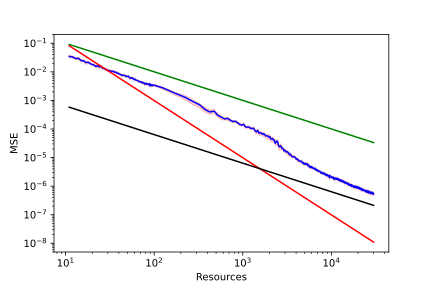
\includegraphics[width=0.5\textwidth]{phaseAndVisibilities/estimation1000010000.pdf}
	\end{center}
	\caption{Plot of the median error of Eq.~\eqref{eq:medianMerit} for the phase only with all the other parameters treated as nuisance parameters, and a confidence interval of 99\% (in light red). The green line is the Standard Quantum Limit $1/N$, and the red one the Heisenberg scaling $1/N^2$. The black line is the reference in Eq.~\eqref{eq:medianCramer} for a weight matrix with only non null entry $G_{11} = 1$.}
	\label{fig:estimation10000}
\end{figure}
%
\begin{figure}[!th]
	\begin{center}
		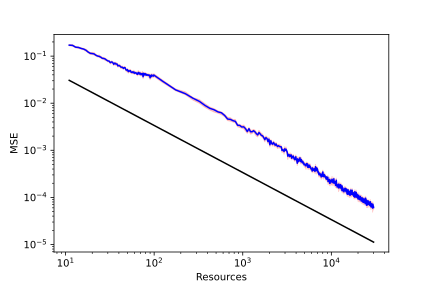
\includegraphics[width=0.5\textwidth]{phaseAndVisibilities/estimation1100011000.pdf}
	\end{center}
	\caption{Plot of the median error of Eq.~\eqref{eq:medianMerit} for the phase and the visibility $V_1$ of the system without active q-plates, with all the other parameters treated as nuisance parameters, and a confidence interval of 99\% (in light red). The black line is the reference in Eq.~\eqref{eq:medianCramer} for a weight matrix with only non null entries $G_{11} = 1$ and $G_{22} = 1$.}	
	\label{fig:estimation11000}
\end{figure}
%
\begin{figure}[!th]
	\begin{center}
		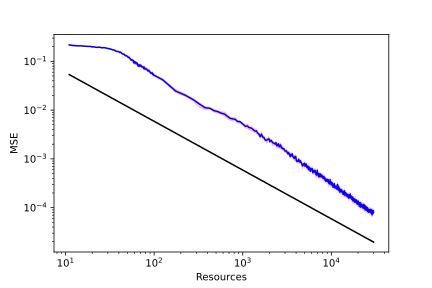
\includegraphics[width=0.5\textwidth]{phaseAndVisibilities/estimation1010010100.pdf}
	\end{center}
	\caption{Plot of the median error of Eq.~\eqref{eq:medianMerit} for the phase and the visibility $V_2$ of the system with the first q-plate active, with all the other parameters treated as nuisance parameters, and a confidence interval of 99\% (in light red). The black line is the reference in Eq.~\eqref{eq:medianCramer} for a weight matrix with only non null entries $G_{11} = 1$ and $G_{33} = 1$.}
	\label{fig:estimation10100}
\end{figure}
%
\begin{figure}[!th]
	\begin{center}
		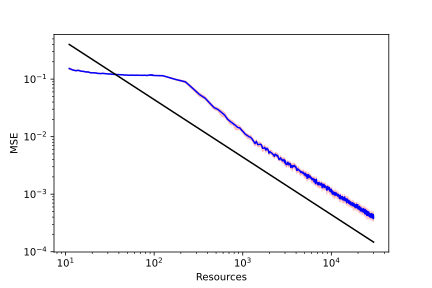
\includegraphics[width=0.5\textwidth]{phaseAndVisibilities/estimation1001010010.pdf}
	\end{center}
	\caption{Plot of the median error of Eq.~\eqref{eq:medianMerit} for the phase and the visibility $V_3$ of the system with the second q-plate active, with all the other parameters treated as nuisance parameters, and a confidence interval of 99\% (in light red). The black line is the reference in Eq.~\eqref{eq:medianCramer} for a weight matrix with only non null entries $G_{11} = 1$ and $G_{44} = 1$.}
	\label{fig:estimation10010}
\end{figure}
%
\begin{figure}[!th]
	\begin{center}
		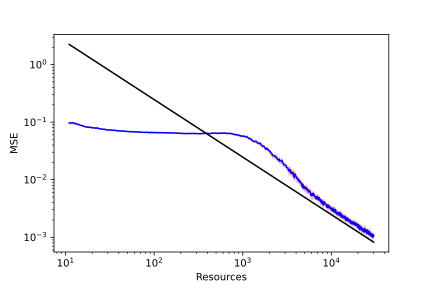
\includegraphics[width=0.5\textwidth]{phaseAndVisibilities/estimation1000110001.pdf}
	\end{center}
	\caption{Plot of the median error of Eq.~\eqref{eq:medianMerit} for the phase and the visibility $V_4$ of the system with the third q-plate active, with all the other parameters treated as nuisance parameters, and a confidence interval of 99\% (in light red). The black line is the reference in Eq.~\eqref{eq:medianCramer} for a weight matrix with only non null entries $G_{11} = 1$ and $G_{55} = 1$.}
	\label{fig:estimation10001}
\end{figure}
%
\begin{figure}[!th]
	\begin{center}
		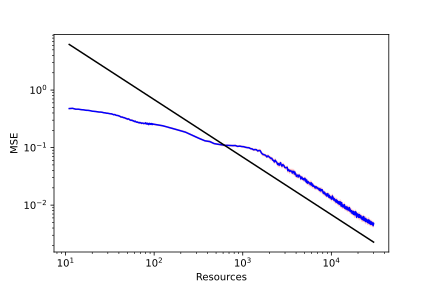
\includegraphics[width=0.5\textwidth]{phaseAndVisibilities/estimation1111111111.pdf}
	\end{center}
	\caption{Plot of the median error of Eq.~\eqref{eq:medianMerit} for the phase and all the visibilities of the system, and a confidence interval of 99\% (in light red). The black line is the reference in Eq.~\eqref{eq:medianCramer} for $G=\id$.}
	\label{fig:estimation11111}
\end{figure}
%

\section{Acknowledgments}
%
The Bayesian data analysis has been programmed with the Python framework PyTorch and ran on a GPU. We gratefully acknowledge computational resources of the Center for High Performance Computing (CHPC) at SNS.
	

\begin{thebibliography}{100}
	
	\bibitem{Cimini2021} V Cimini \textit{et al.}, \href{http://arxiv.org/abs/2110.02908}{arXiv:2110.02908 (2021).}
	%
	
	\bibitem{Granade2012} C E Granade \textit{et al.} 2012 \href{https://doi.org/10.1088/1367-2630/14/10/103013}{New J. Phys. {\bf 14} 103013}.
	%
	
	%\bibitem{Roccia2018} E Roccia \textit{et al.}, \href{https://www.osapublishing.org/optica/abstract.cfm?uri=optica-5-10-1171}{Optica~{\bf 5}, 1171-1176 (2018).}
	%
	
	\bibitem{Belliardo2020} F Belliardo and V Giovannetti, \href{https://link.aps.org/doi/10.1103/PhysRevA.102.042613}{Phys. Rev. A~{\bf 102}, 042613}.
	%
	

	
\end{thebibliography}

\end{document}